%%\documentclass[draft]{article}
\documentclass[12pt]{article}
\usepackage[cp1251]{inputenc}
\usepackage[english]{babel}

\usepackage{amssymb,amsthm,amsmath}
\usepackage{graphicx}

\textwidth=17cm \oddsidemargin=-5mm \topmargin=-20mm
\textheight=25cm
\renewcommand{\baselinestretch}{1.5}

\tolerance=10000

\begin{document}

\begin{center}
Ordena\c{c}\~ao usando formulas de Excel
\end{center}

\begin{abstract}
Columna A de plalinha conten os valores num\'ericos, que devem ser
ordenados em outra columna, usando somente as fun\c{c}\~oes e
Excel. N\'os propormos essa ordena\c{c}c\~ao usando somente as
func\c{c}\~oes: SE, INDIRETO, CONCATENAR, LINHA, \`EERROS,
CORRESP.
\end{abstract}


\section{Descri\c{c}\~ao de problema}

Suponha a columna $A$ tem n\'umeros, que comesam as A2 (deichamos
a primeira linha para coment\'arios etc.). Preenchemos as celulas
de $A$ com formulas

\begin{figure}[htb]
\begin{center}
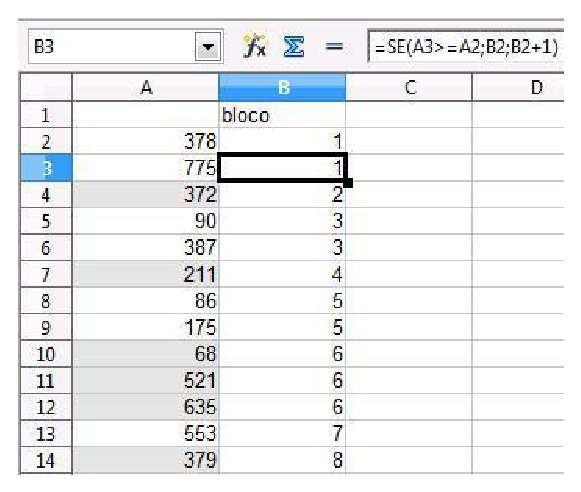
\includegraphics{./imgs/pic1}
\end{center}
\caption{}
\end{figure}

\centerline{=ALEAT\`ORIOENTRE(0;\, 1000)}

\noindent para os testes futuros. Vamos adicionar a columna $B$
com as formulas seguintes:

B1:\, 1

B2:\, =SE(A3\textgreater =A2;B2;B2+1)

Copiamos B2 para baixo.\\

Assim, escrevemos na columna B as n\'umeros de blocos ordenados de
columna A. Se columna A \'e ordenda, crescente, todos os valores
do B ser\~ao 1s. No caso contr\'ario A precisa uma
permuta\c{c}\~ao para ser ordenada. Mais d'isso, podemos usar
columna B para formata\c{c}\~ao condicional do A.



Vamos colocar nas columnas C e D os n\'umeros de linhas, cujas
elementos vamos comparar, juntando os blocos ordenados.

\begin{figure}[htb]
\begin{center}
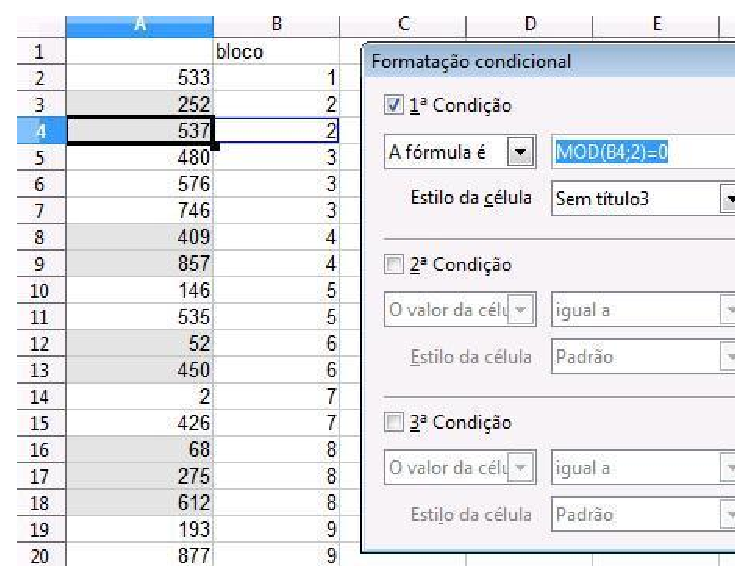
\includegraphics{./imgs/pic2}
\end{center}
\caption{}
\end{figure}

Vamos explicar pelo exemplo. Seja na columna A temos blocos
ordenados $\{63,\, 193, 438\}$ e $\{241,\, 372\}$. Para juntar
esses blocos devemos fazer as conpera\c{c}\~oes seguintes:

\begin{figure}[htb]
\begin{center}
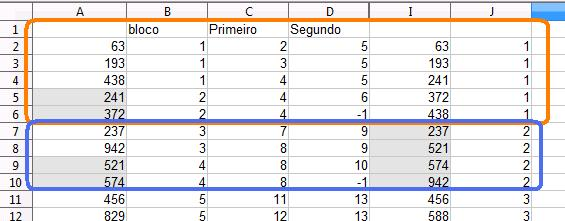
\includegraphics{./imgs/pic3}
\end{center}
\caption{}\label{pic3}
\end{figure}

$$
\begin{array}{lllll}
\{63,\, 193, 438\}& \{241,\, 372\}& 63 * 241 &\longrightarrow &
63;\\
\{193, 438\}& \{241,\, 372\}& 193 * 241 &\longrightarrow& 193
\\
\{438\}& \{241,\, 372\}& 438 * 241 &\longrightarrow & 241;
\\
\{438\}& \{372\}& 438 * 372& \longrightarrow& 372;
\\
\{438\}& \{\emptyset \}& 438 * \{\emptyset\}& \longrightarrow&
438;
\end{array}$$

For os valores de conjuntos $\{63,\, 193, 438\}$ e $\{241,\,
372\}$ s\~ao armasenados nos campos $\{ A2,\, A3,\, A4\}$ e $\{
A5,\, A6\}$, podemos reescrever a sequ\"encia de opera\c{c}\~oes
de ordena\c{c}\~ao na maneira seguinte:

$$
\begin{array}{lllll}
\multicolumn{5}{c}{\{A2=63,\, A3=193, A4=438\};\ \{A5=241,\,
A6=372\}}\\
\{A2,\, A3, A4\}& \{A5,\, A6\}& A2 * A5 &\longrightarrow &
A2;\\
\{ A3, A4\}& \{A5,\, A6\}& A3 * A5 &\longrightarrow& A3
\\
\{ A4\}& \{A5,\, A6\}& A4 * A5 &\longrightarrow & A5;
\\
\{ A4\}& \{A6\}& A4 * A6& \longrightarrow& 372;
\\
\{  A4\}& \{\emptyset \}& A4 * \{\emptyset\}& \longrightarrow& A4;
\end{array}$$

Retangulo lagange de Fig.~\ref{pic3} descibe o processo de
ordena\c{c}\~ao de pare mencionada de duas sequ\"encias ordenadas.
Por exemplo, linha 4 corresponde a compara\c{c}\~ao $$ \{A4 * A5
\longrightarrow \  A5 =241\}.
$$

Assim, nossa tarefa de jun\c{c}\~ao de conjuntos $\{63,\, 193,
438\}$ e $\{241,\, 372\}$ precisa determina\c{c}\~ao de elementos
de columnas C e D. Lembramos, que os conjuntos $\{63,\, 193,
438\}$ e $\{241,\, 372\}$ er\~ao de exemplos, mas tamanho deles
n\~ao \'e dado, e deve ser computado pelas formulas com columns A
\'unica entrada.

\section{Resolu\c{c}\~ao}

\textbf{Come\c{c}o de proximo bloco ordenado}. Pelo como
contruirmos planilha, o primeiro bloco ordenado com\c{c}a em A2.

para essa dinalidade usamos a func\c{c}\~ao \textbf{CORRESP}.\\

\noindent\textbf{CORRESP}(valor\_procurado, matriz\_procurada,
[tipo\_correspondencia]).\\
Tipo\_correspondencia=0 localiza o
primeiro valor que e exatamente igual a valor\_procurado.\\

Com columna B, podemos procurar o come\c{c}o de proximo bloco como

\centerline{=CORRESP(B2+1;B\$2:B\$31;0)}

\noindent lembrando que os valores para ordenar fiacam em A2:A31,
e os n\'umeros de blcos ordenados est\~ao em B2:B31.

Assim, prrenchemos as celulas C2 e D2 com:

C2:\ =LINHA(B2)

D2:\ =1+CORRESP(B2+1;B\$2:B\$31;0)\\

\textbf{Recuperar valor ordenado pelo n\'umero de columna}. Para
esse finalidade vamos usar composi\c{c}\~ao de fun\c{c}\~oes
INDIRETO e CONCATENAR.

Fun\c{c}\~ao INDIRETO devolve o valor de c\'elula elo seu
argunento. Por exemplo, INDIRETO("A5") devolva o valor (texto ou
numero) de celula A5.

Fun\c{c}\~ao CONCATENAR concatena seus argumentos. Por exemplo, se
H10 contem o n\'umero 15, ent\~ao

\centerline{=INDIRETO(CONCATENAR("A";\, H10))}

\noindent vai devolver o conteudo de A15. Assim, como na
Figura~\ref{pic3}, devemos comparar os valores de A, com indices
de C2 e D2, a expre\c{c}\~ao correspondente \'e

\centerline{=INDIRETO(CONCATENAR("A";\, C2))\textless
INDIRETO(CONCATENAR("A";\, D2))}

Quando guntamos dois conjuntos ordenados, vai acontecer um
momento, quando um desses conjuntos vai acabar. Nesse caso
escrevemos no correspondente valor ``-1" de columna C ou D. Assim,
vamos comparar os valores com n\'umeros em C10 e D10 como

\noindent
=\textbf{SE}(C10=-1;\, D10;\\
\phantom{=\textbf{SE}(}\textbf{SE}(D10=-1;\, C10;\\
\phantom{=\textbf{SE}(\textbf{SE}( }\textbf{SE}(\textbf{INDIRETO}(
\textbf{CONCATENAR}( ``A";\, C10))\textless
=\\
\phantom{=\textbf{SE}(\textbf{SE}(\textbf{SE}(aaa
}\textbf{INDIRETO}( \textbf{CONCATENAR}(``A";\, D10));\\
\phantom{=\textbf{SE}(\textbf{SE}(\textbf{SE}( }C10;\, D10)))

Vamos colocar essa compara\c{c}\~ao na columna E.

Vamos colocar nas columnas F e G os indicadores de fato, que n\~ao
h\'a o proximo elemento de primeiro ou segundo conjunto
respetivamente.

Essas formalas, para linha 10, ser\~ao as seguintes:

\noindent
F10:\\
=\textbf{SE}( C10=-1;\,
0=0;\\
\phantom{=\textbf{SE}( }\textbf{INDIRETO}(\textbf{CONCATENAR}(``B";C10))\textless\textgreater\\
\phantom{=\textbf{SE}(
aaa}\textbf{INDIRETO}(\textbf{CONCATENAR}(``B";C10+1)))

\noindent
G10:\\
=\textbf{SE}(D10=-1;0=0;\\
\phantom{=\textbf{SE}(
}\textbf{INDIRETO}(\textbf{CONCATENAR}(``B";D10))\textless\textgreater\\
\phantom{=\textbf{SE}(
aaa}\textbf{INDIRETO}(\textbf{CONCATENAR}(``B";D10+1)))


\begin{figure}[htb]
\begin{center}
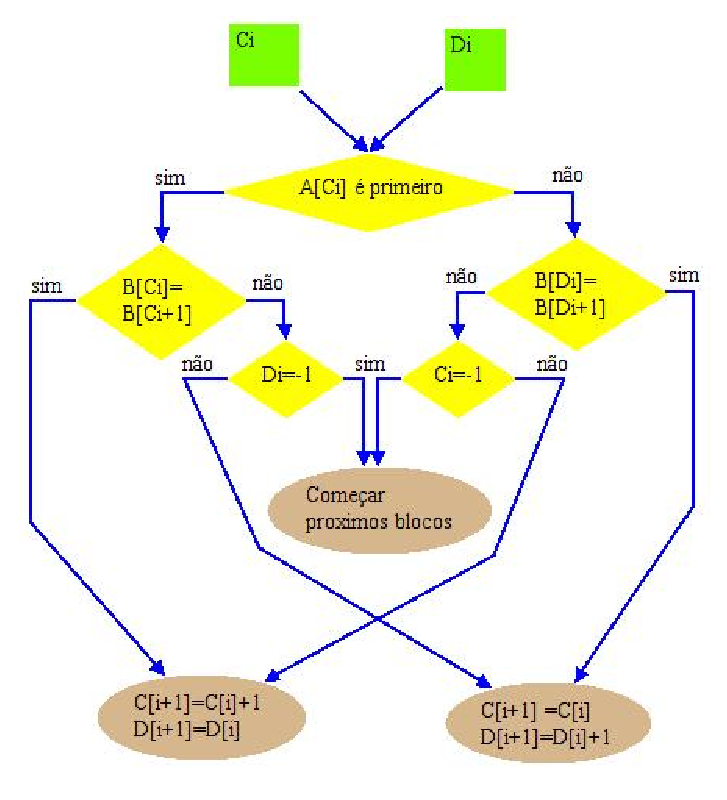
\includegraphics{./imgs/pic4}
\end{center}
\caption{}\label{pic4}
\end{figure}

\textbf{Proxima pare de elementos para comparar}.

O fluxograma de algoritimo de constu\c{c}\~ao de valores de C[i+1]
e D[i+1] pelas Ci e Di est\'a dada na Fig.~\ref{pic4}. Com essa
fluxigrama podemos construir as formulas para columnas C e D.

Vamos usar uma columna auxiliar H para o proximo valor (linha para
columna D) no caso, se temos um come\c{c}o de novo conjunto. Essa
express\~ao ser\'a similar \`a aquela de celula D2, mas com uma
pequena complica\c{c}\~ao. Pode acontecer, que o conunto em
columna A \'e \'ultmo e, assim, n\~ao h\'a o n\'umero de conjunto
proximo. Nesse caso a fun\c{c}\~ao \textbf{CORRESP} vai devolver
um erro \#N/A. Devemos prender esse erro, e develver -1 no caso.
Assim, temos uma formaula para celula H10:

\noindent
H10:\\
=\textbf{SE}(\textbf{\'EERROS}(1+\textbf{CORRESP}(B10+1;B\$2:B\$31;0));\\
\phantom{=\textbf{SE}(}-1;\\
\phantom{=\textbf{SE}(}1+\textbf{CORRESP}(B10+1;B\$2:B\$31;0))

Vamos usar columna H e diagrama de Fig.~\ref{pic4} para formulas
de columnas C e~D.

\noindent
C10:\\
=\textbf{SE}(C9=E9;\\
\phantom{=\textbf{SE}(}\textbf{SE}(F9;\\
\phantom{=\textbf{SE}(\textbf{SE}(}\textbf{SE}(D9\textless\textgreater
-1;\, -1;\, \textbf{LINHA}(B10));\\
\phantom{=\textbf{SE}(\textbf{SE}(}C9+1);\\
\phantom{=\textbf{SE}(} \textbf{SE}(C9\textless\textgreater -1;\,
C9;\, \textbf{SE}(G9;\textbf{LINHA}(B10);-1)))

\noindent
D10:\\
=\textbf{SE}(D9=E9;\\
\phantom{=\textbf{SE}(}\textbf{SE}(G9;\\
\phantom{=\textbf{SE}(\textbf{SE}(}
\textbf{SE}(C9\textless\textgreater -1;\, -1;\,
\textbf{SE}(F9;H10;-1));\\
\phantom{=\textbf{SE}(\textbf{SE}(}
D9+1);\\
\phantom{=\textbf{SE}(} \textbf{SE}(D9\textless\textgreater -1;\,
D9;\, \textbf{SE}(F9;H10;D9)))

\begin{figure}[htb]
\begin{center}
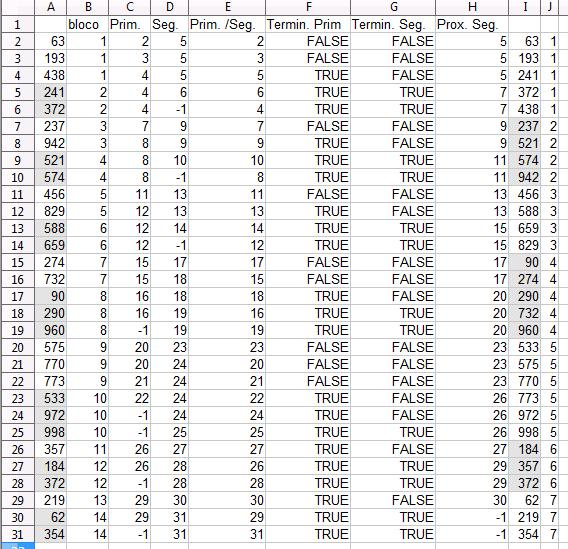
\includegraphics{./imgs/pic5}
\end{center}
\caption{}\label{pic5}
\end{figure}

Assim, constiuirmos mais a columna I pela columna A, cuntando
pares dos blocos subsequentes ordenados de A, e diminuindo a
quantidade de blocos ordenados aproximadamente duas vezes (veja
Fig.~\ref{pic5}).\\

Vamos \textbf{melhorar as formulas desenvolvidas}. Lembramos, que
quando usamos a composi\c{c}\~ao
``\textbf{INDIRETO}(\textbf{CONCATENAR}...'', usamos o nome de
columna (A ou B) explicito. Isto atrapnlha a possibilidade de
copiar essas formulas. A fun\c{c}\~ao \textbf{INDIRETO} aceita o
argumento tamb\'em na maneira RiCj, de acrecentas o segundo
algumento ``FALSE". Por exemplo,

\centerline{=INDIRETO("R1C2";1=0)}

\noindent devolva o valor ``bloco'', que est\'a na celula B2, cuja
linha (``R'' \'e de palavra ingles ``row'')\'e 1, e columna \'e 2
(``R'' \'e de palavra ingles ``column'').

Assim, usando esse jeuito de fun\c{c}\~ao INDIRETO, podemos
re-escrever as formulas de columnas E, F, G, H, I na maneira
seguinte:

E10:\\
=\textbf{SE}(\\
\phantom{=\textbf{SE}(}C10=-1;\\
\phantom{=\textbf{SE}(}D10;\\
\phantom{=\textbf{SE}(}\textbf{SE}(D10=-1;\\
\phantom{=\textbf{SE}(\textbf{SE}(}
C10;\\
\phantom{=\textbf{SE}(\textbf{SE}(
}\textbf{SE}(\textbf{INDIRETO}(\textbf{CONCATENAR}(
``R";C10;``C";\textbf{COLUNA}(A10));0)\textless
=\\
\phantom{=\textbf{SE}(\textbf{SE}(\textbf{SE}(}
\textbf{INDIRETO}(\textbf{CONCATENAR}(``R";D10;``C";
\textbf{COLUNA}(A10));0);\\
\phantom{=\textbf{SE}(\textbf{SE}(\textbf{SE}(}C10;D10)))

F10:\\
=\textbf{SE}(\\
\phantom{=\textbf{SE}(}C10=-1;0=0;\\
\phantom{=\textbf{SE}(}\textbf{INDIRETO}(
\textbf{CONCATENAR}(``R";C10;``C";\textbf{COLUNA}(B10));0)
\textless\textgreater\\
\phantom{=\textbf{SE}(aaa} \textbf{INDIRETO}(\textbf{CONCATENAR}(
``R";C10+1;``C";\textbf{COLUNA}(B10));0))

\begin{figure}[htb]
\begin{center}
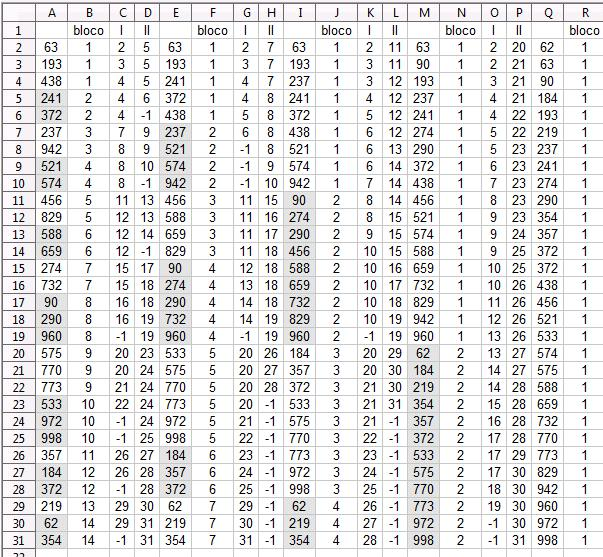
\includegraphics{./imgs/pic6}
\end{center}
\caption{}\label{pic6}
\end{figure}

G10:\\
=\textbf{SE}(D10=-1;0=0;\\
\phantom{=\textbf{SE}(} \textbf{INDIRETO}(
\textbf{CONCATENAR}(``R";D10;``C";\textbf{COLUNA}(B10));0)
\textless\textgreater\\
\phantom{=\textbf{SE}(aaa} \textbf{INDIRETO}(
\textbf{CONCATENAR}(``R";D10+1;``C";\textbf{COLUNA}(B10));0))

H10:\\
=\textbf{SE}(\\
\phantom{=\textbf{SE}(}\textbf{\'EERROS}(1
+\textbf{CORRESP}(B10+1;B\$2:B\$31;0));\\
\phantom{=\textbf{SE}(}-1;\\
\phantom{=\textbf{SE}(}1 +\textbf{CORRESP}(B10+1;B\$2:B\$31;0))

I10:\\
=\textbf{INDIRETO}(\textbf{CONCATENAR}(
``R";E10;``C";\textbf{COLUNA}(A10));0)\\

Podemos \textbf{elminimal as columnas auxiliadoras} E, F, G, e H.
Isto signigica, que vamos copiar as formulas dessas columnas para
cada lugar, onde essas formulas s\~ao mencionadas. Depois dessa
elimina\c{c}\~ao obtemoas as formulas seguintes:

C2:\\
LINHA(B2)

C3:\\
SE(C2=SE(C2=-1;D2;SE(D2=-1;C2;SE( INDIRETO(CONCATENAR(``R";C2;``C";\\
COLUNA(A2));0)\textless=INDIRETO( CONCATENAR(``R";D2;``C";
COLUNA(A2)); 0); C2;\\
D2) )); SE(SE(C2=-1;0=0; INDIRETO(
 CONCATENAR(``R";C2;``C";\\
 COLUNA(B2));0)\textless\textgreater INDIRETO(CONCATENAR(``R";C2+1;``C";
COLUNA(B2));0));SE(D2\textless\textgreater
-1;-1;LINHA(B3));C2+1);SE(C2\textless\textgreater -1;C2;SE(SE(D2=
-1;0=0;INDIRETO( CONCATENAR(``R";D2;``C";
COLUNA(B2));0)\textless\textgreater\\
INDIRETO( CONCATENAR(``R";D2+1;``C";
COLUNA(B2));0));LINHA(B3);-1)))

Deve copiar C3 at\'e fim da lista.

D2:\\
1+CORRESP(B2+1;B\$2:B\$31;0)

D3:\\
{SE}( D2={SE}( C2=-1; D2; SE( D2=-1; C2; SE(
{INDIRETO}( {CONCATENAR}(\\
``R"; C2; ``C"; \mbox{{COLUNA}}(A2)); 0) \textless=
{INDIRETO}( {CONCATENAR}(``R";\\
D2; ``C"; \mbox{{COLUNA}}(A2) ); 0); C2; D2))); SE( SE(
D2=-1; 0=0; {INDIRETO}(\\
{CONCATENAR}(``R"; D2; ``C";
\mbox{{COLUNA}}(B2));0)\textless\textgreater
{INDIRETO}( {CONCATENAR}(\\
``R";D2+1;``C"; \mbox{{COLUNA}}(B2));0)); SE( C2
\textless\textgreater -1;-1;SE(SE(C2=-1;0=0; {INDIRETO}(\\
{CONCATENAR}( ``R"; C2;``C"; \mbox{{COLUNA}}(B2));0)
\textless\textgreater {INDIRETO}(\\
{CONCATENAR}(``R"; C2+1;``C";
\mbox{{COLUNA}}(B2));0));SE({\'EERROS}( 1
+\\
{CORRESP}( B3+1;B\$2:B\$31;0)); -1; 1+{CORRESP}(
B3+1;B\$2:B\$31;0));-1)); D2+1);\\
SE( D2\textless\textgreater -1; D2;SE( SE(C2=-1;0=0;
{INDIRETO}( {CONCATENAR}(\\
``R";C2;``C"; {COLUNA}(B2));0)\textless\textgreater
{INDIRETO}( {CONCATENAR}(\\
``R";C2+1;``C"; {COLUNA}(B2));0));\\
{SE}( {\'EERROS}( 1+{CORRESP}(B3+1;\\
B\$2:B\$31; 0));-1; 1 +{CORRESP}(B3+1; B\$2:B\$31; 0)); D2)))


Deve copiar D3 at\'e fim da lista.

E2:\\
INDIRETO(CONCATENAR(``R";SE(C2=-1;D2;SE(D2=-1;C2;
SE(INDIRETO(CONCATENAR(``R";C2;``C";COLUNA(A2));0)
\textless=\\
INDIRETO(CONCATENAR(``R";D2;``C";COLUNA(A2));0);C2;D2)));\\
``C";COLUNA(A2));0)

Deve copiar E2 at\'e fim da lista.

Depois de todas essas opera\c{c}\~oes podemos copiar as
computa\c{c}\~oes para direiro, aplicaldo-les para columnas
obtidas na cada passo, at\'e finalizar ordena\c{c}\~ao. O
resultado dessas aplica\c{c}\~oes est\' na Fig.~\ref{pic6}.

\end{document}
